\documentclass{article}

\usepackage{polski}
\usepackage[utf8]{inputenc}
\usepackage{graphicx}
\usepackage{amsfonts}
\usepackage{amssymb}
\usepackage{amsmath}
\usepackage{listings}
\usepackage{breqn}
\usepackage{float}

\author{Maciej Pieta \and Piotr Koproń \and Jakub Woś \and Rafał Piwowar}
\date{Marzec 2023}

\title{Technika Cyfrowa. \\ Ćwiczenie 2.}

\begin{document}
\maketitle
\newpage

\section{Zadanie 2a}
\paragraph{Treść zadania} Na podstawie dostępnych tabel prawdy, zaprojektować i praktycznie zrealizować synchroniczny przerzutnik D w oparciu o dostępny synchroniczny przerzutnik T, po czym proszę jednoznacznie przetestować poprawność jego działania w programie Multisim. 
\subsection{Ogólna idea rozwiązania}
\begin{figure}[H]
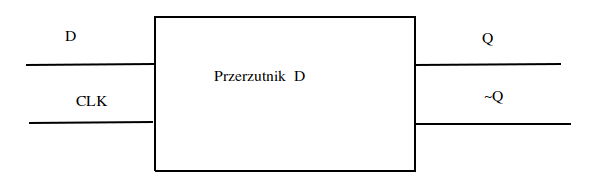
\includegraphics[width=0.7\textwidth]{DBB}
\end{figure}
Jako że realizacja ma opierać się o synchroniczny przerzutnik T, to schemat przyjmuje postać:
\begin{figure}[H]
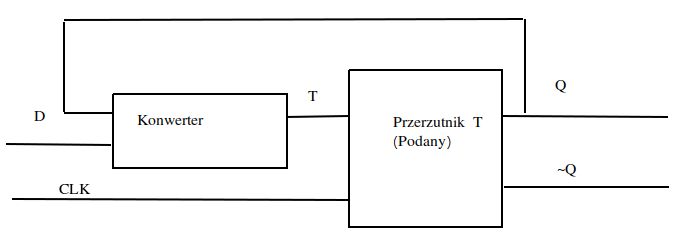
\includegraphics[width=0.7\textwidth]{KBB}
\end{figure}
W celu wyznaczenia bramek logicznych zastosujemy następujący algorytm: \\
1. Wyznaczymy wzory przejścia dla przerzutników D oraz T.
2. Nadamy równoważność wzorom przejścia.
3. Otrzymamy zależność między sygnałami D,T, oraz Q.
4. Przekształcimy otrzymaną zależność do funkcji T od D i Q.
\newpage
\paragraph{Wzory przejścia}
Dla przerzutnika T: \\
\begin{tabular}{c c c}
T & Q & $Q_{T}^{+}$ \\
0 & 0 & 0 \\
0 & 1 & 1 \\
1 & 0 & 1 \\
1 & 1 & 0
\end{tabular}
$\implies$ Z definicji xor otrzymujemy $Q^{+} = T \text{ xor } Q$. (1) \\
Dla przerzutnika D: \\
\begin{tabular}{c c c}
D & Q & $Q_{D}^{+}$ \\
0 & 0 & 0 \\
0 & 1 & 0 \\
1 & 0 & 1 \\
1 & 1 & 1
\end{tabular}
$\implies $ Bezpośrednio otrzymujemy $Q_{D} = D$. (2)\\
Z (1) i (2) otrzymujemy równoważność $D = T \text{ xor } Q$ (3).
\paragraph{Przekształcenie do funkcji}
Chcemy utworzyć funkcję T od D i Q, tak aby (3) zawsze było spełnione. Tworzymy tabelę, gdzie po lewej stronie będziemy mieć wartości niezależne, po prawej - wyrażenia zależne.
\begin{center}
\begin{tabular}{c c c | c c }
D & Q & $D = T \text{ xor } Q$ & $T \text{ xor } Q$ & T \\
0 & 0 & 1 & 0 & 0\\
0 & 1 & 1 & 0 & 1\\
1 & 0 & 1 & 1 & 1\\
1 & 1 & 1 & 1 & 0
\end{tabular}
\end{center}
Usuwając kolumny $D = T \text{ xor } Q$ i $T \text{ xor } Q$ z powyższej tabeli, otrzymujemy:
\begin{tabular}{c c c }
D & Q & T \\
0 & 0 & 0\\
0 & 1 & 1\\
1 & 0 & 1\\
1 & 1 & 0
\end{tabular} $\implies$ Z definicji xor otrzymujemy $ T = D \text{ xor } Q$. \\

\section{Zadanie 2b}

\end{document}